\documentclass[conference]{IEEEtran}

\usepackage{cite}
\usepackage{amsmath,amssymb,amsfonts}
\usepackage{algorithm}
\usepackage{algorithmic}
\usepackage{graphicx}
\graphicspath{{../figures/}{figures/}}
\usepackage{textcomp}
\usepackage{xcolor}
\usepackage{booktabs}
\usepackage{array}

\def\BibTeX{{\rm B\kern-.05em{\sc i\kern-.025em b}\kern-.08em
    T\kern-.1667em\lower.7ex\hbox{E}\kern-.125emX}}

\begin{document}

\title{Adaptive Restart Particle Swarm Optimization Based on Search Resource Reallocation}

\author{
    \IEEEauthorblockN{1\textsuperscript{st} Chenshuo Cai}
    \IEEEauthorblockA{
        \textit{Xinyang Normal University}\\
        Xinyang, China\\
        caichenshuo@foxmail.com
    }
    \and
    \IEEEauthorblockN{2\textsuperscript{nd} Zhongyang Chen*}
    \IEEEauthorblockA{
        \textit{Xinyang Normal University}\\
        Xinyang, China\\
        czy112@xynu.edu.cn\\
        *Corresponding author
    }
}

\maketitle

\begin{abstract}
    Particle swarm optimization (PSO) is easy to implement, but its particles may still spend many function evaluations around a locally attractive region after the swarm has lost diversity. This work studies that behavior as a problem of search resource use rather than only as a parameter-tuning issue. An adaptive restart particle swarm optimizer based on search resource reallocation, called ARPSO-SRR, is developed. The algorithm monitors stagnation and normalized population diversity, estimates restart intensity from the current search state, and reallocates selected low-contribution particles through a mixture of global regeneration and local perturbation near the current best solution. A more detailed inefficient-particle identification variant is kept as an ablation case, so that the effect of a heavier selection rule can be checked separately from the main restart framework. Tests are carried out on the available functions of the CEC2017 benchmark suite with 30 independent runs for each function. The experimental results show that ARPSO-SRR gives a clear improvement over standard PSO and several PSO variants on many functions with limited runtime overhead. Differential evolution and comprehensive learning PSO still obtain stronger overall ranks, but ARPSO-SRR offers a compact restart-based improvement for the PSO family.
\end{abstract}

\begin{IEEEkeywords}
    particle swarm optimization, adaptive restart, hybrid restart, search resource reallocation, numerical optimization
\end{IEEEkeywords}

\section{Introduction}
Particle swarm optimization (PSO) is a population-based metaheuristic motivated by collective behavior \cite{b1}. In a standard PSO search, each particle is guided by its own best experience and by the best position discovered by the whole swarm. Because this update rule is short and requires only a few parameters, PSO remains a common choice for continuous black-box optimization problems.

The same simplicity also leads to a familiar weakness. When most particles are pulled into a narrow region too early, the swarm may keep evaluating very similar candidate points. The algorithm is still spending the evaluation budget, but part of that budget is no longer producing useful exploration. In this paper, this situation is treated as a search resource allocation problem: particles that repeatedly search redundant regions should be redirected before the remaining evaluations are wasted.

Existing PSO improvements usually address this issue from different angles. Adaptive inertia weights change the step tendency during the run \cite{b2}. Stability and constriction studies explain how the swarm dynamics can be controlled \cite{b3}. Comprehensive learning PSO (CLPSO) reduces premature convergence by making particles learn from different exemplars \cite{b4}. Restart-based methods are more direct: they move part of the population when the current search state becomes unproductive.

For restart-based PSO, the key difficulty is not only whether to restart. A fixed restart ratio may be too weak for a collapsed swarm and too disruptive when useful local exploitation is still ongoing. A restart operator also has to decide whether new particles should be sent to unexplored areas or kept near the best region already found. These two choices motivate an adaptive and hybrid restart design.

This paper proposes ARPSO-SRR, an adaptive restart PSO based on search resource reallocation. The method uses stagnation and diversity information to decide when a restart is needed, adjusts the restart intensity according to the search state, and combines global random regeneration with local perturbation around the current best solution. The basic PSO update is retained, so the proposed method can be implemented without changing the main optimization framework.

The contributions are as follows:
\begin{itemize}
    \item A restart-based PSO framework is formulated from the perspective of reallocating evaluation resources away from stagnated or redundant particles.
    \item An adaptive restart intensity rule is used so that the number of restarted particles changes with stagnation length and population diversity.
    \item A hybrid restart operator combines global regeneration and local perturbation, allowing the restart process to recover diversity while still using information from promising regions.
    \item A six-variant ablation study and a comparison with standard PSO, PSO variants, GA, DE, and CLPSO are conducted on the available CEC2017 functions, using average ranks, convergence curves, restart behavior, runtime, and nonparametric statistical tests.
\end{itemize}

\section{Related Work}\label{sec:related}

\subsection{Standard Particle Swarm Optimization}
Let $x_i^t$ and $v_i^t$ denote the position and velocity of particle $i$ at iteration $t$. The velocity and position update equations of standard PSO are
\begin{equation}
    v_i^{t+1}=w v_i^t+c_1 r_1(p_i^t-x_i^t)+c_2 r_2(g^t-x_i^t),
    \label{eq:pso_velocity}
\end{equation}
\begin{equation}
    x_i^{t+1}=x_i^t+v_i^{t+1},
    \label{eq:pso_position}
\end{equation}
where $w$ is the inertia weight, $c_1$ and $c_2$ are acceleration coefficients, $r_1$ and $r_2$ are uniformly sampled random numbers, $p_i^t$ is the personal best position, and $g^t$ is the global best position.

The update in (1) makes the swarm converge by combining historical self-learning and social learning. In practical runs, however, this mechanism can also amplify attraction to a local region. Once the swarm radius becomes very small, changing only the velocity parameters may not be enough to create new search directions.

\subsection{Adaptive and Learning-Based Variants}
Adaptive PSO variants change inertia weights or acceleration coefficients during the search, so that exploration and exploitation are not controlled by a single fixed setting \cite{b2,b12}. HPSO-TVAC follows this idea by varying acceleration coefficients over time \cite{b11}. CLPSO modifies the learning structure more substantially: dimensions of a particle can learn from different exemplars, which usually helps preserve population diversity on multimodal landscapes \cite{b4}.

These variants show that PSO performance is sensitive to how search information is shared. The present work uses them as baselines, but it takes a different path. Instead of replacing the velocity model, ARPSO-SRR keeps the standard PSO update and intervenes only when the current population distribution suggests that some particles are no longer contributing enough.

\subsection{Restart Strategies}
Restart strategies are commonly used to recover exploration after stagnation \cite{b13,b14}. A basic restart may randomly regenerate particles after several iterations without improvement. More elaborate designs may select particles by poor fitness, crowding, distance from the best solution, or individual improvement history.

In ARPSO-SRR, restart is interpreted as resource reallocation. A restarted particle gives up an unproductive trajectory and uses its future evaluations at a new position. Under this view, the restart module should specify the trigger, the number of particles to reallocate, and the way those particles are regenerated. The proposed method is built around these three choices.

\section{Proposed Method}\label{sec:method}

\subsection{Motivation and Overall Framework}
In the proposed framework, a particle is viewed not only as a candidate solution but also as a carrier of future function evaluations. When several particles stay close to one another and stop improving, keeping all of them in the same region is unlikely to provide much new information. ARPSO-SRR therefore reallocates a controlled part of the swarm after stagnation or diversity loss has been detected.

The framework has three connected steps. The first step records stagnation and normalized diversity. The second step converts these indicators into a restart demand value and then into the number of particles to be restarted. The third step regenerates the selected particles using both global and local restart operators. Fig.~\ref{fig:framework} gives the overall procedure.

\begin{figure}[!t]
    \centering
    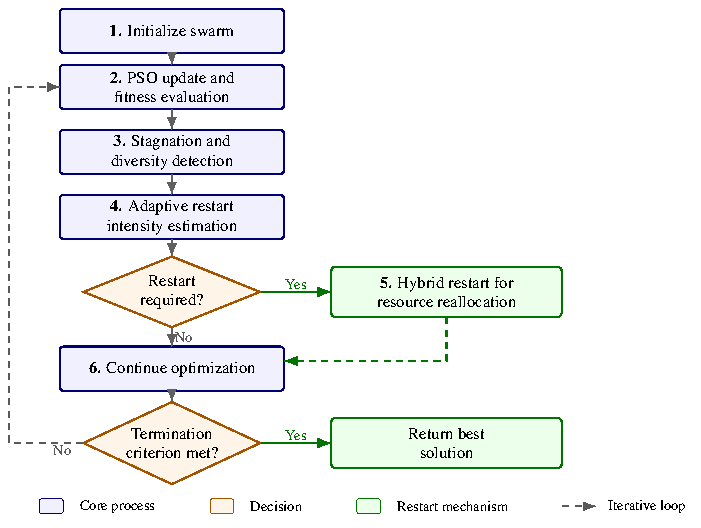
\includegraphics[width=\linewidth]{framework_tikz_final.pdf}
    \caption{Framework of the proposed ARPSO-SRR.}
    \label{fig:framework}
\end{figure}

\subsection{Stagnation and Diversity Detection}
Population diversity is measured after boundary normalization, so the threshold does not depend directly on the coordinate scale of a benchmark function. Each particle is first mapped into the normalized search space:
\begin{equation}
    \tilde{x}_i^t=\frac{x_i^t-l}{u-l},
    \label{eq:normalized_position}
\end{equation}
where $l$ and $u$ are the lower and upper bounds of the search space, and the division is performed element-wise. The normalized diversity is then defined as
\begin{equation}
    D^t=\frac{1}{N\sqrt{d}}\sum_{i=1}^{N}
    \left\|\tilde{x}_i^t-\bar{\tilde{x}}^t\right\|_2,
    \label{eq:diversity}
\end{equation}
where $N$ is the population size, $d$ is the problem dimension, and $\bar{\tilde{x}}^t$ is the center of the normalized swarm. A low $D^t$ value means that the particles occupy only a small part of the feasible search range.

Fitness stagnation is counted by the number of consecutive iterations in which the global best solution is not improved. Let $s^t$ denote this count. A restart is triggered when $s^t\ge s_{\mathrm{thr}}$ or $D^t\le D_{\mathrm{thr}}$, where the two thresholds are listed in Table~\ref{tab:parameters}. Using both criteria avoids relying on fitness history alone, since a population can become highly concentrated even before a long stagnation period is observed.

\subsection{Adaptive Restart Intensity}
The restart ratio is not fixed in ARPSO-SRR. It is calculated from the current search condition as follows:
\begin{equation}
    \rho^t=\rho_{\min}+(\rho_{\max}-\rho_{\min})Q^t,
    \label{eq:restart_ratio}
\end{equation}
where $\rho_{\min}$ and $\rho_{\max}$ are the lower and upper bounds of the restart ratio, and $Q^t$ is a normalized restart demand indicator. In this study, $Q^t$ is computed by
\begin{equation}
    \begin{aligned}
        q_s^t & = \min\left(1,\frac{s^t}{3s_{\mathrm{thr}}}\right),                 \\
        q_D^t & = \max\left(0,\frac{D_{\mathrm{thr}}-D^t}{D_{\mathrm{thr}}}\right), \\
        Q^t   & = \max(q_s^t,q_D^t),
    \end{aligned}
    \label{eq:restart_demand}
\end{equation}
Here, $q_s^t$ increases with stagnation length and $q_D^t$ increases when the normalized diversity falls below the threshold. The larger of the two values is used as the restart demand. The number of restarted particles is then obtained by
\begin{equation}
    m^t=\left\lceil \rho^t N \right\rceil .
    \label{eq:restart_number}
\end{equation}

After $m^t$ is obtained, particles are selected with a lightweight score. The current global-best particle is protected from restart, and all other particles are ranked by
\begin{equation}
    R_i=0.65R_i^{fit}+0.35R_i^{stag},
    \label{eq:srr_selection}
\end{equation}
where $R_i^{fit}$ is the min--max normalized fitness disadvantage and $R_i^{stag}$ is the min--max normalized individual no-improvement length. The top $m^t$ particles are restarted. This selection rule is intentionally compact; the paper focuses on adaptive restart intensity and hybrid regeneration, while the more complex inefficient-particle score is kept only for ablation comparison.

As a result, the restart strength changes gradually. Weak stagnation leads to a small reallocation, whereas severe stagnation or diversity loss restarts a larger part of the swarm.

\subsection{Hybrid Restart Strategy}
Selected particles are regenerated by two operators. The global operator samples new positions from the full feasible region:
\begin{equation}
    x_i^{t+1}=l+(u-l)\odot r,
    \label{eq:global_restart}
\end{equation}
where $l$ and $u$ are the lower and upper bounds, $r$ is a uniformly sampled random vector, and $\odot$ denotes element-wise multiplication. This operator is used to restore broad exploration.

The local operator perturbs particles around the current global best:
\begin{equation}
    x_i^{t+1}=g^t+\sigma^t (u-l)\odot z,
    \label{eq:local_restart}
\end{equation}
where $g^t$ is the current global best position, $z$ is a random vector, and $\sigma^t$ is the perturbation scale. The scale is bounded by $\sigma_{\min}$ and $\sigma_{\max}$ and decreases during the run, so the local restart is wider early in the search and narrower near the end.

The mixed design is used to avoid two undesirable cases. A fully global restart may ignore useful information already gathered near the best region, while a fully local restart may not restore enough diversity. Splitting the restarted particles between the two operators gives a practical compromise.

\subsection{Algorithm Procedure}
Algorithm~\ref{alg:arpso_srr} summarizes the procedure. Standard PSO updates are performed first. The restart module is then called only when the stagnation or diversity criterion is satisfied.

\begin{algorithm}[!t]
    \caption{ARPSO-SRR}
    \label{alg:arpso_srr}
    \begin{algorithmic}[1]
        \STATE Initialize particle positions $x_i$ and velocities $v_i$
        \STATE Evaluate particles and initialize $p_i$ and $g$
        \STATE Initialize stagnation counter and diversity record
        \WHILE{termination criterion is not satisfied}
        \STATE Update velocities using \eqref{eq:pso_velocity}
        \STATE Update positions using \eqref{eq:pso_position}
        \STATE Repair particles that exceed the search bounds
        \STATE Evaluate particles and update $p_i$ and $g$
        \STATE Measure normalized diversity $D^t$ using \eqref{eq:diversity}
        \STATE Update stagnation counter $s^t$
        \IF{restart condition is satisfied}
        \STATE Calculate restart ratio $\rho^t$ using \eqref{eq:restart_ratio}
        \STATE Determine restart number $m^t$ using \eqref{eq:restart_number}
        \STATE Select particles using \eqref{eq:srr_selection}
        \STATE Apply global random regeneration to part of selected particles
        \STATE Apply local perturbation around $g$ to remaining selected particles
        \STATE Repair restarted particles that exceed the search bounds
        \STATE Evaluate restarted particles and update $p_i$ and $g$
        \STATE Reset stagnation-related records
        \ENDIF
        \ENDWHILE
        \STATE \textbf{return} best solution $g$
    \end{algorithmic}
\end{algorithm}

\subsection{Boundary Handling and Evaluation Accounting}
After a standard update or a restart step, each coordinate is clipped to the feasible interval $[l,u]$ before evaluation. Restarted particles consume function evaluations in the same budget as all other evaluated particles, and their personal bests and the global best are updated using the standard PSO rule. This setting avoids giving the proposed method extra evaluations.

\subsection{Complexity Analysis}
The standard velocity and position update costs $O(Nd)$ per iteration. The diversity measurement in \eqref{eq:diversity} has the same order, and the restart operation also costs at most $O(Nd)$ when all particles are considered. The priority score in \eqref{eq:srr_selection} only uses population-level statistics. Thus, ARPSO-SRR keeps the same asymptotic order as standard PSO, with only a small additional constant cost. The evaluation budget is unchanged.

\section{Experimental Setup}\label{sec:experiment}

\subsection{Benchmark Functions}
The experiments use the CEC2017 single-objective real-parameter benchmark suite \cite{b5}. In the adopted implementation, F2 is unavailable; therefore, the tested set contains F1 and F3--F30, giving 29 functions in total. The dimension is fixed at $d=30$, and the maximum number of function evaluations (FEs) is $10{,}000d$, namely 300,000 evaluations per run.

These functions cover unimodal, simple multimodal, hybrid, and composition landscapes. The grouping used in the later analysis is shown in Table~\ref{tab:function_groups}.

\begin{table}[!t]
    \caption{CEC2017 Function Groups Used in the Experiments}
    \centering
    \begin{tabular}{cc}
        \toprule
        Group             & Functions \\
        \midrule
        Unimodal          & F1, F3    \\
        Simple multimodal & F4--F10   \\
        Hybrid            & F11--F20  \\
        Composition       & F21--F30  \\
        \bottomrule
    \end{tabular}
    \label{tab:function_groups}
\end{table}

\subsection{Compared Algorithms and Parameters}
Eight algorithms are used for comparison: standard PSO, PSO with adaptive inertia weight (PSO-AW), PSO with random restart (PSO-RS), CLPSO, HPSO-TVAC, genetic algorithm (GA) \cite{b6}, differential evolution (DE) \cite{b7}, and ARPSO-EIS. ARPSO-EIS denotes a variant with a more explicit inefficient-particle identification rule, and it is included to test whether that extra selection complexity is beneficial.

Each algorithm is run 30 times independently on every tested function. The population size is set to 50 for all algorithms, and the same maximum FE budget is used throughout the comparison. The GA crossover and mutation rates are 0.80 and 0.10. The DE parameters are $F=0.50$ and $CR=0.90$. Other settings are listed in Table~\ref{tab:parameters}.

\begin{table}[!t]
    \caption{Experimental Parameter Settings}
    \centering
    \footnotesize
    \setlength{\tabcolsep}{2.5pt}
    \resizebox{\columnwidth}{!}{%
        \begin{tabular}{ll}
            \toprule
            Parameter                  & Setting                                     \\
            \midrule
            Dimension                  & 30                                          \\
            Population size            & 50                                          \\
            Maximum FEs                & 300,000                                     \\
            Independent runs           & 30                                          \\
            Benchmark functions        & CEC2017 F1, F3--F30                         \\
            Compared algorithms        & 9                                           \\
            Inertia weight range       & $w_{\max}=0.9$, $w_{\min}=0.4$              \\
            Acceleration coefficients  & $c_1=2.0$, $c_2=2.0$                        \\
            Velocity clamp ratio       & 0.20                                        \\
            Stagnation threshold       & 50 iterations                               \\
            Diversity threshold        & 0.05                                        \\
            Restart ratio range        & $\rho_{\min}=0.08$, $\rho_{\max}=0.40$      \\
            Restart demand             & \eqref{eq:restart_demand}                   \\
            Global/local restart ratio & 0.50 / 0.50                                 \\
            Local perturbation range   & $\sigma_{\min}=0.002$, $\sigma_{\max}=0.06$ \\
            \bottomrule
        \end{tabular}%
    }
    \label{tab:parameters}
\end{table}

\subsection{Evaluation Metrics}
For each run, the final optimization error is recorded. The analysis reports the mean value, standard deviation, average rank, runtime, and restart statistics. Average ranks are calculated from the final errors on each benchmark function. The Friedman test is used for the overall multi-algorithm comparison, and the Wilcoxon signed-rank test is used for pairwise comparisons between ARPSO-SRR and each competitor \cite{b8,b9,b10}. The significance level is 0.05.

\section{Results and Discussion}\label{sec:results}

\subsection{Ablation Study}
Table~\ref{tab:ablation} gives the six-variant ablation results on the 28 functions for which complete ablation records are available. This part is used to study the restart design itself; the overall algorithm comparison in the next subsections still uses the 29-function benchmark set. A lower average rank is better. ARPSO-SRR and ARPSO-Local both obtain an average rank of 2.71, while ARPSO-EIS and ARPSO-Fixed are tied behind them. The result suggests that the proposed adaptive hybrid design reaches the best ablation rank without relying only on an aggressive local restart.

\begin{table}[!t]
    \caption{Six-Variant Ablation Results on the Functions with Complete Ablation Records}
    \centering
    \footnotesize
    \setlength{\tabcolsep}{2pt}
    \resizebox{\columnwidth}{!}{%
        \begin{tabular}{lcccc}
            \toprule
            Algorithm    & Avg. rank & Avg. restarts & Rest. particles & Runtime (s) \\
            \midrule
            ARPSO-Local  & 2.71      & 3561.7        & 33812.2         & 118.24      \\
            ARPSO-SRR    & 2.71      & 2229.8        & 14847.4         & 118.42      \\
            ARPSO-EIS    & 3.46      & 2048.1        & 13273.5         & 119.40      \\
            ARPSO-Fixed  & 3.46      & 1626.6        & 16265.6         & 116.87      \\
            ARPSO-Global & 4.25      & 1538.4        & 10613.0         & 116.63      \\
            PSO-RS       & 4.39      & 1324.9        & 8633.6          & 116.13      \\
            \bottomrule
        \end{tabular}%
    }
    \label{tab:ablation}
\end{table}

The restart counts show why the two tied variants should not be interpreted as equivalent. ARPSO-Local triggers 3561.7 restart events on average and replaces 33812.2 particles. ARPSO-SRR triggers 2229.8 events and replaces 14847.4 particles. Thus, ARPSO-Local replaces about 2.28 times as many particles as ARPSO-SRR. The proposed variant reaches the same average rank while using a noticeably smaller restart scale.

Fig.~\ref{fig:ablation} shows the same ranking pattern visually. Together with Table~\ref{tab:ablation}, the figure highlights the main trade-off: ARPSO-SRR reaches the tied best average rank, but it restarts far fewer particles than the purely local restart variant.

\begin{figure}[!t]
    \centering
    
\includegraphics[width=\linewidth]{ablation6_average_rank.pdf}
    \caption{Ablation comparison of the six restart variants on the completed ablation functions. Lower average rank indicates better performance.}
    \label{fig:ablation}
\end{figure}

The Friedman test over the 28-function ablation set gives a statistic of 21.6596 and $p=6.08\times 10^{-4}$, so the restart design has a measurable effect on performance. Pairwise Wilcoxon counts are more conservative: ARPSO-SRR obtains 6/22/0 win/non-significant-difference/loss counts against PSO-RS, 8/19/1 against ARPSO-Global, 5/22/1 against ARPSO-EIS, and 1/24/3 against ARPSO-Local. These results do not show universal dominance. Rather, they support the intended trade-off between performance and restart cost.

\subsection{Overall Performance}
Table~\ref{tab:rank_runtime} summarizes the overall average rank and runtime. Lower rank values indicate better final errors, and the relative runtime is normalized by the runtime of ARPSO-SRR.

\begin{table}[!t]
    \caption{Average Rank and Runtime of Compared Algorithms}
    \centering
    \footnotesize
    \setlength{\tabcolsep}{2pt}
    \resizebox{\columnwidth}{!}{%
        \begin{tabular}{cccc}
            \toprule
            Algorithm & Avg. rank & Avg. runtime (s) & Rel. runtime to ARPSO-SRR \\
            \midrule
            DE        & 1.97      & 89.88            & 1.25                      \\
            CLPSO     & 3.17      & 77.40            & 1.08                      \\
            GA        & 4.21      & 85.44            & 1.19                      \\
            ARPSO-SRR & 4.31      & 71.82            & 1.00                      \\
            ARPSO-EIS & 4.45      & 72.07            & 1.00                      \\
            HPSO-TVAC & 5.34      & 72.82            & 1.01                      \\
            PSO-RS    & 6.07      & 76.21            & 1.06                      \\
            PSO       & 7.55      & 74.09            & 1.03                      \\
            PSO-AW    & 7.93      & 75.37            & 1.05                      \\
            \bottomrule
        \end{tabular}%
    }
    \label{tab:rank_runtime}
\end{table}

DE obtains the best overall rank, and CLPSO and GA follow. ARPSO-SRR ranks fourth among the nine algorithms. This is a useful position for the proposed method: it is weaker than strong nonrestart or learning-based competitors, but it is clearly ahead of standard PSO, PSO-AW, PSO-RS, and HPSO-TVAC in average rank. Its average runtime is 71.82 seconds, lower than those of CLPSO, GA, and DE in this experiment. The restart module therefore adds little overhead in the adopted setting.

\subsection{Function-group Analysis}
Table~\ref{tab:group_rank} breaks the ranks down by function group, which helps identify where the restart mechanism is more useful.


\begin{table}[!t]
    \caption{Average Rank of Representative Algorithms on Different Function Groups}
    \centering
    \footnotesize
    \setlength{\tabcolsep}{2pt}
    \resizebox{\columnwidth}{!}{%
        \begin{tabular}{lcccccc}
            \toprule
            Group             & PSO-RS & HPSO-TVAC & CLPSO & GA   & DE   & ARPSO-SRR \\
            \midrule
            Unimodal          & 5.00   & 6.50      & 2.50  & 6.50 & 1.50 & 3.00      \\
            Simple multimodal & 6.71   & 4.00      & 2.57  & 6.00 & 3.43 & 4.86      \\
            Hybrid            & 6.10   & 4.90      & 3.40  & 3.30 & 1.10 & 4.80      \\
            Composition       & 5.80   & 6.50      & 3.50  & 3.40 & 1.90 & 3.70      \\
            \bottomrule
        \end{tabular}%
    }
    \label{tab:group_rank}
\end{table}

The clearest group-level result for ARPSO-SRR appears on composition functions, where its average rank is 3.70. This indicates that adaptive restart can help when the landscape contains several interacting components. On simple multimodal and hybrid functions, CLPSO and DE remain stronger, so ARPSO-SRR should be regarded as a PSO-family enhancement rather than a general replacement for these baselines.

\subsection{Convergence and Restart Behavior}
Fig.~\ref{fig:convergence} presents the mean error curves on CEC2017-F23. On this composition function, ARPSO-SRR continues to reduce the error after the early phase and finishes below PSO and PSO-RS. DE still gives the lowest final error, which is consistent with the overall ranking in Table~\ref{tab:rank_runtime}.

\begin{figure}[!t]
    \centering
    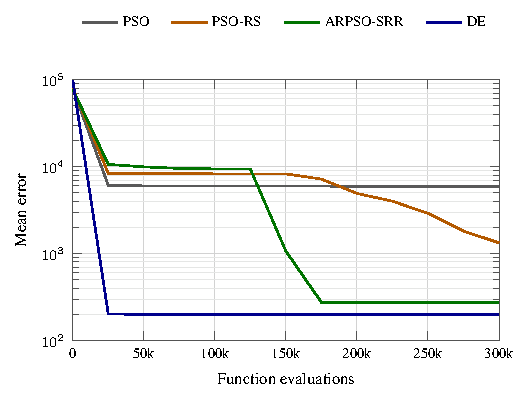
\includegraphics[width=\linewidth]{convergence_curve_tikz_final.pdf}
    \caption{Representative convergence behavior on CEC2017-F23.}
    \label{fig:convergence}
\end{figure}

Fig.~\ref{fig:restart_behavior} plots the mean restart ratio of ARPSO-SRR on CEC2017-F23 over 30 runs. The ratio is almost zero at the beginning and rises later, after the swarm has spent a substantial part of the budget. This pattern matches the design goal: restart should be limited early and become more active when stagnation or diversity loss appears. Over the 29-function experiment, ARPSO-SRR records 67.72 restarts on average, compared with 8.94 for PSO-RS.

\begin{figure}[!t]
    \centering
    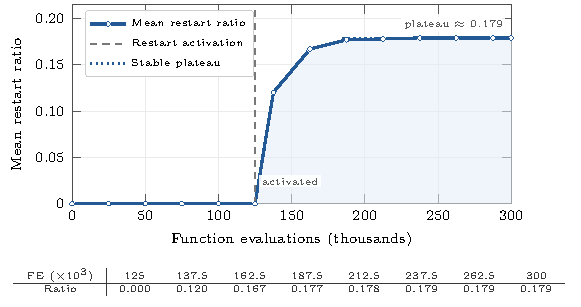
\includegraphics[width=\linewidth]{restart_behavior_tikz_final.pdf}
    \caption{Mean restart ratio of ARPSO-SRR on CEC2017-F23 over 30 independent runs.}
    \label{fig:restart_behavior}
\end{figure}

\subsection{Statistical Analysis}
The Friedman test over the 29 benchmark functions gives a statistic of 117.2414 with $p=1.2296\times10^{-21}$. Thus, the compared algorithms do not have the same overall rank distribution.

\begin{table}[!t]
    \caption{Friedman Test over All Compared Algorithms}
    \centering
    \begin{tabular}{cccc}
        \toprule
        Statistic & $p$-value              & Functions & Algorithms \\
        \midrule
        117.2414  & $1.2296\times10^{-21}$ & 29        & 9          \\
        \bottomrule
    \end{tabular}
    \label{tab:friedman}
\end{table}

Table~\ref{tab:wilcoxon} gives the Wilcoxon signed-rank summary for ARPSO-SRR against each competitor. ``Win'', ``NSD'', and ``Loss'' count functions where ARPSO-SRR is significantly better, not significantly different, or significantly worse, respectively.

\begin{table}[!t]
    \caption{Wilcoxon Signed-rank Test Summary for ARPSO-SRR}
    \centering
    \begin{tabular}{cccc}
        \toprule
        Compared algorithm & Win & NSD & Loss \\
        \midrule
        PSO                & 17  & 11  & 1    \\
        PSO-AW             & 19  & 10  & 0    \\
        PSO-RS             & 17  & 11  & 1    \\
        HPSO-TVAC          & 13  & 9   & 7    \\
        GA                 & 11  & 9   & 9    \\
        ARPSO-EIS          & 1   & 27  & 1    \\
        CLPSO              & 7   & 6   & 16   \\
        DE                 & 3   & 3   & 23   \\
        \bottomrule
    \end{tabular}
    \label{tab:wilcoxon}
\end{table}

The pairwise results are consistent with the rank table. ARPSO-SRR records many wins against PSO, PSO-AW, and PSO-RS, and it has more wins than losses against HPSO-TVAC. The comparison with GA is roughly balanced. CLPSO and DE are stronger, with ARPSO-SRR losing on more functions. Against ARPSO-EIS, the 1/27/1 result shows that the more complex inefficient-particle selection rule does not provide a stable advantage in this experiment.


\subsection{Discussion}
Overall, the experiments support the use of ARPSO-SRR as a lightweight improvement to PSO-family algorithms. The method is not the strongest optimizer in the comparison, and the results against CLPSO and DE show that exemplar learning and differential mutation remain very competitive. Nevertheless, ARPSO-SRR improves clearly over standard PSO, adaptive-weight PSO, and simple random restart PSO. The ablation results further suggest that the benefit comes from controlled resource reallocation rather than from restarting as many particles as possible. A future version should make the trigger and restart intensity more problem-adaptive, especially for hybrid functions where the current ranks are still modest.


\section{Conclusion}\label{sec:conclusion}
This paper presented ARPSO-SRR, an adaptive restart PSO algorithm designed around search resource reallocation. The method monitors stagnation and normalized diversity, changes the restart intensity according to the observed search state, and uses both global regeneration and local perturbation under the original function-evaluation budget.

The experiments on the available CEC2017 functions show that ARPSO-SRR improves over standard PSO, PSO-AW, and PSO-RS on many functions. The statistical tests and average ranks also show the method's limitation: DE and CLPSO remain stronger overall baselines. The comparison with ARPSO-EIS suggests that adding a heavier inefficient-particle identification rule is not enough to bring stable extra improvement. Future work will focus on more adaptive restart triggers, large-scale settings, and real-world optimization tasks.


\begin{thebibliography}{00}
    \bibitem{b1} J. Kennedy and R. Eberhart, ``Particle swarm optimization,'' in \textit{Proc. IEEE Int. Conf. Neural Networks (ICNN)}, Perth, WA, Australia, 1995, pp. 1942--1948, doi: 10.1109/ICNN.1995.488968.

    \bibitem{b2} Y. Shi and R. Eberhart, ``A modified particle swarm optimizer,'' in \textit{Proc. IEEE Int. Conf. Evolutionary Computation (ICEC)}, Anchorage, AK, USA, May 1998, pp. 69--73, doi: 10.1109/ICEC.1998.699146.

    \bibitem{b3} M. Clerc and J. Kennedy, ``The particle swarm---explosion, stability, and convergence in a multidimensional complex space,'' \textit{IEEE Trans. Evol. Comput.}, vol. 6, no. 1, pp. 58--73, Feb. 2002, doi: 10.1109/4235.985692.

    \bibitem{b4} J. J. Liang, A. K. Qin, P. N. Suganthan, and S. Baskar, ``Comprehensive learning particle swarm optimizer for global optimization of multimodal functions,'' \textit{IEEE Trans. Evol. Comput.}, vol. 10, no. 3, pp. 281--295, Jun. 2006, doi: 10.1109/TEVC.2005.857610.

    \bibitem{b5} N. H. Awad, M. Z. Ali, P. N. Suganthan, J. J. Liang, and B. Y. Qu, ``Problem definitions and evaluation criteria for the CEC 2017 special session and competition on single objective real-parameter numerical optimization,'' Nanyang Technological Univ., Singapore, Tech. Rep., 2016.

    \bibitem{b6} J. H. Holland, \textit{Adaptation in Natural and Artificial Systems}. Ann Arbor, MI, USA: Univ. of Michigan Press, 1975.

    \bibitem{b7} R. Storn and K. Price, ``Differential evolution---a simple and efficient heuristic for global optimization over continuous spaces,'' \textit{J. Global Optim.}, vol. 11, no. 4, pp. 341--359, Dec. 1997, doi: 10.1023/A:1008202821328.

    \bibitem{b8} F. Wilcoxon, ``Individual comparisons by ranking methods,'' \textit{Biometrics Bull.}, vol. 1, no. 6, pp. 80--83, Dec. 1945, doi: 10.2307/3001968.

    \bibitem{b9} M. Friedman, ``The use of ranks to avoid the assumption of normality implicit in the analysis of variance,'' \textit{J. Amer. Stat. Assoc.}, vol. 32, no. 200, pp. 675--701, Dec. 1937, doi: 10.1080/01621459.1937.10503522.

    \bibitem{b10} J. Derrac, S. Garc\'{i}a, D. Molina, and F. Herrera, ``A practical tutorial on the use of nonparametric statistical tests as a methodology for comparing evolutionary and swarm intelligence algorithms,'' \textit{Swarm Evol. Comput.}, vol. 1, no. 1, pp. 3--18, Mar. 2011, doi: 10.1016/j.swevo.2011.02.002.

    \bibitem{b11} A. Ratnaweera, S. K. Halgamuge, and H. C. Watson, ``Self-organizing hierarchical particle swarm optimizer with time-varying acceleration coefficients,'' \textit{IEEE Trans. Evol. Comput.}, vol. 8, no. 3, pp. 240--255, Jun. 2004, doi: 10.1109/TEVC.2004.826071.

    \bibitem{b12} Z.-H. Zhan, J. Zhang, Y. Li, and H. S.-H. Chung, ``Adaptive particle swarm optimization,'' \textit{IEEE Trans. Syst., Man, Cybern. B, Cybern.}, vol. 39, no. 6, pp. 1362--1381, Dec. 2009, doi: 10.1109/TSMCB.2009.2015956.

    \bibitem{b13} J. Gou, Y.-X. Lei, W.-P. Guo, C. Wang, Y.-Q. Cai, and W. Luo, ``A novel improved particle swarm optimization algorithm based on individual difference evolution,'' \textit{Appl. Soft Comput.}, vol. 57, pp. 468--481, Aug. 2017, doi: 10.1016/j.asoc.2017.04.025.

    \bibitem{b14} L. Liu, H. Xu, B. Wang, R. Zhang, and J. Chen, ``A study on particle swarm algorithm based on restart strategy and adaptive dynamic mechanism,'' \textit{Electronics}, vol. 11, no. 15, Art. no. 2339, Jul. 2022, doi: 10.3390/electronics11152339.
\end{thebibliography}

\end{document}
